\documentclass[ngerman,compress,hyperref={bookmarks}]{beamer}
\usetheme{Antibes}
\useoutertheme{infolines}

\usepackage[T1]{fontenc}
\usepackage[utf8x]{inputenc}

\usepackage{multirow}

\usepackage{colortbl}
\definecolor{dunkelgrau}{rgb}{0.8, 0.8, 0.8}

\usepackage{wasysym}

\logo{\includegraphics[height=1cm]{images/logoHAW}}
\usepackage{graphicx}

\title[Aktive Messverfahren z. Topologievalidierung]{Aktive Messverfahren zur Topologievalidierung\\ im Routing-Atlas}
\subtitle{Vortrag: Ringvorlesung Seminar}
\subject{Routing-Atlas, Topology}
\author{Andreas Krohn}
\institute[HAW]{Hochschule für Angewandte Wissenschaften Hamburg}
\date[WS 2012/13]{14. November 2012}

\begin{document}
\frame[plain]{\titlepage}

\section*{Agenda}
\begin{frame}{Agenda} \setcounter{tocdepth}{1} \tableofcontents[part=1] \setcounter{tocdepth}{3} \end{frame}

\part{Hauptteil}
\section{Intro}
\subsection{Motivation}
\begin{frame}{Motivation}
  \begin{itemize}
    \item Internet ist kritische Infrastruktur
    \item Bestrebungen zur Kontrolle (Gesetzgeber, Contentindustrie,\ldots)
    \item Topologie nicht komplett bekannt
    \item Beteiligte nicht komplett bekannt
  \end{itemize}
\end{frame}

\subsection{Ziel}
\begin{frame}{Ziel}
  Entwicklung eines Analysewerkzeugs % „Routing-Atlas“
  \begin{itemize}
    \item Zuordnung von Akteuren zu Ländern
    \item Modellierung der Topologie
    \item Visualisierung
  \end{itemize}
\end{frame}

\subsection{Routing-Atlas}
\begin{frame}{Routing-Atlas}
  Ein Projekt der inet AG in Kooperation mit dem BSI
\end{frame}

\section{Rückblick}
\subsection{AW 1}
\begin{frame}{Anwendungen 1}
  Vorstellung des Projekts Routing-Atlas\\
  \begin{itemize}
    \item Identifikation des „deutschen Internets“
    \item Bildung des AS Graphen
    \item Visualisierung
  \end{itemize}
  \vspace{0.5cm}
  Ziel\\
  \begin{itemize}
    \item Ersatz für next hop matrix von Winter
  \end{itemize}
\end{frame}

\subsection{AW2}
\begin{frame}{Anwendungen 2 - Related Work}
  Vorstellung vergleichbarer Arbeiten
  \begin{itemize}
    \item Passive Messverfahren:
  \end{itemize}
\end{frame}

\section{Work in Progress}
\subsection{Projekt1}
\begin{frame}[allowframebreaks]{Projekt1}
  Ursprüngliches Ziel: Aktualisierung der Topologiemodellierung
  \begin{itemize}
    \item Versuchsweise Implementierung von single- und all-pair-shortest-path Algorithmen
    \item Untersuchung zu Laufzeitverhalten und Speicherverbrauch
    \item Fazit: Es gibt Tools, die das besser können\\
    \hspace{0.2cm}z.B. \url{http://www.r-project.org/}
  \end{itemize}
  \framebreak

  Jetzt: Validierung und Ergänzung der Topologiemodellierung
\end{frame}


\section{Ausblick}
\begin{frame}{Ausblick}
\end{frame}

\part{Ende}
\section{kthxbye}
\begin{frame}[plain]{Ende}
\begin{columns}[t]
\begin{column}{0.5\textwidth}
 \begin{center}
 \vspace{1cm}
 Vielen Dank für die Aufmerksamkeit\\
 \vspace{1.5cm}
 Fragen\ldots?
 \end{center}
\end{column}
\begin{column}{0.5\textwidth}
 \vspace{-1cm}
%  \begin{figure}
%   \label{asngraphs2}
%   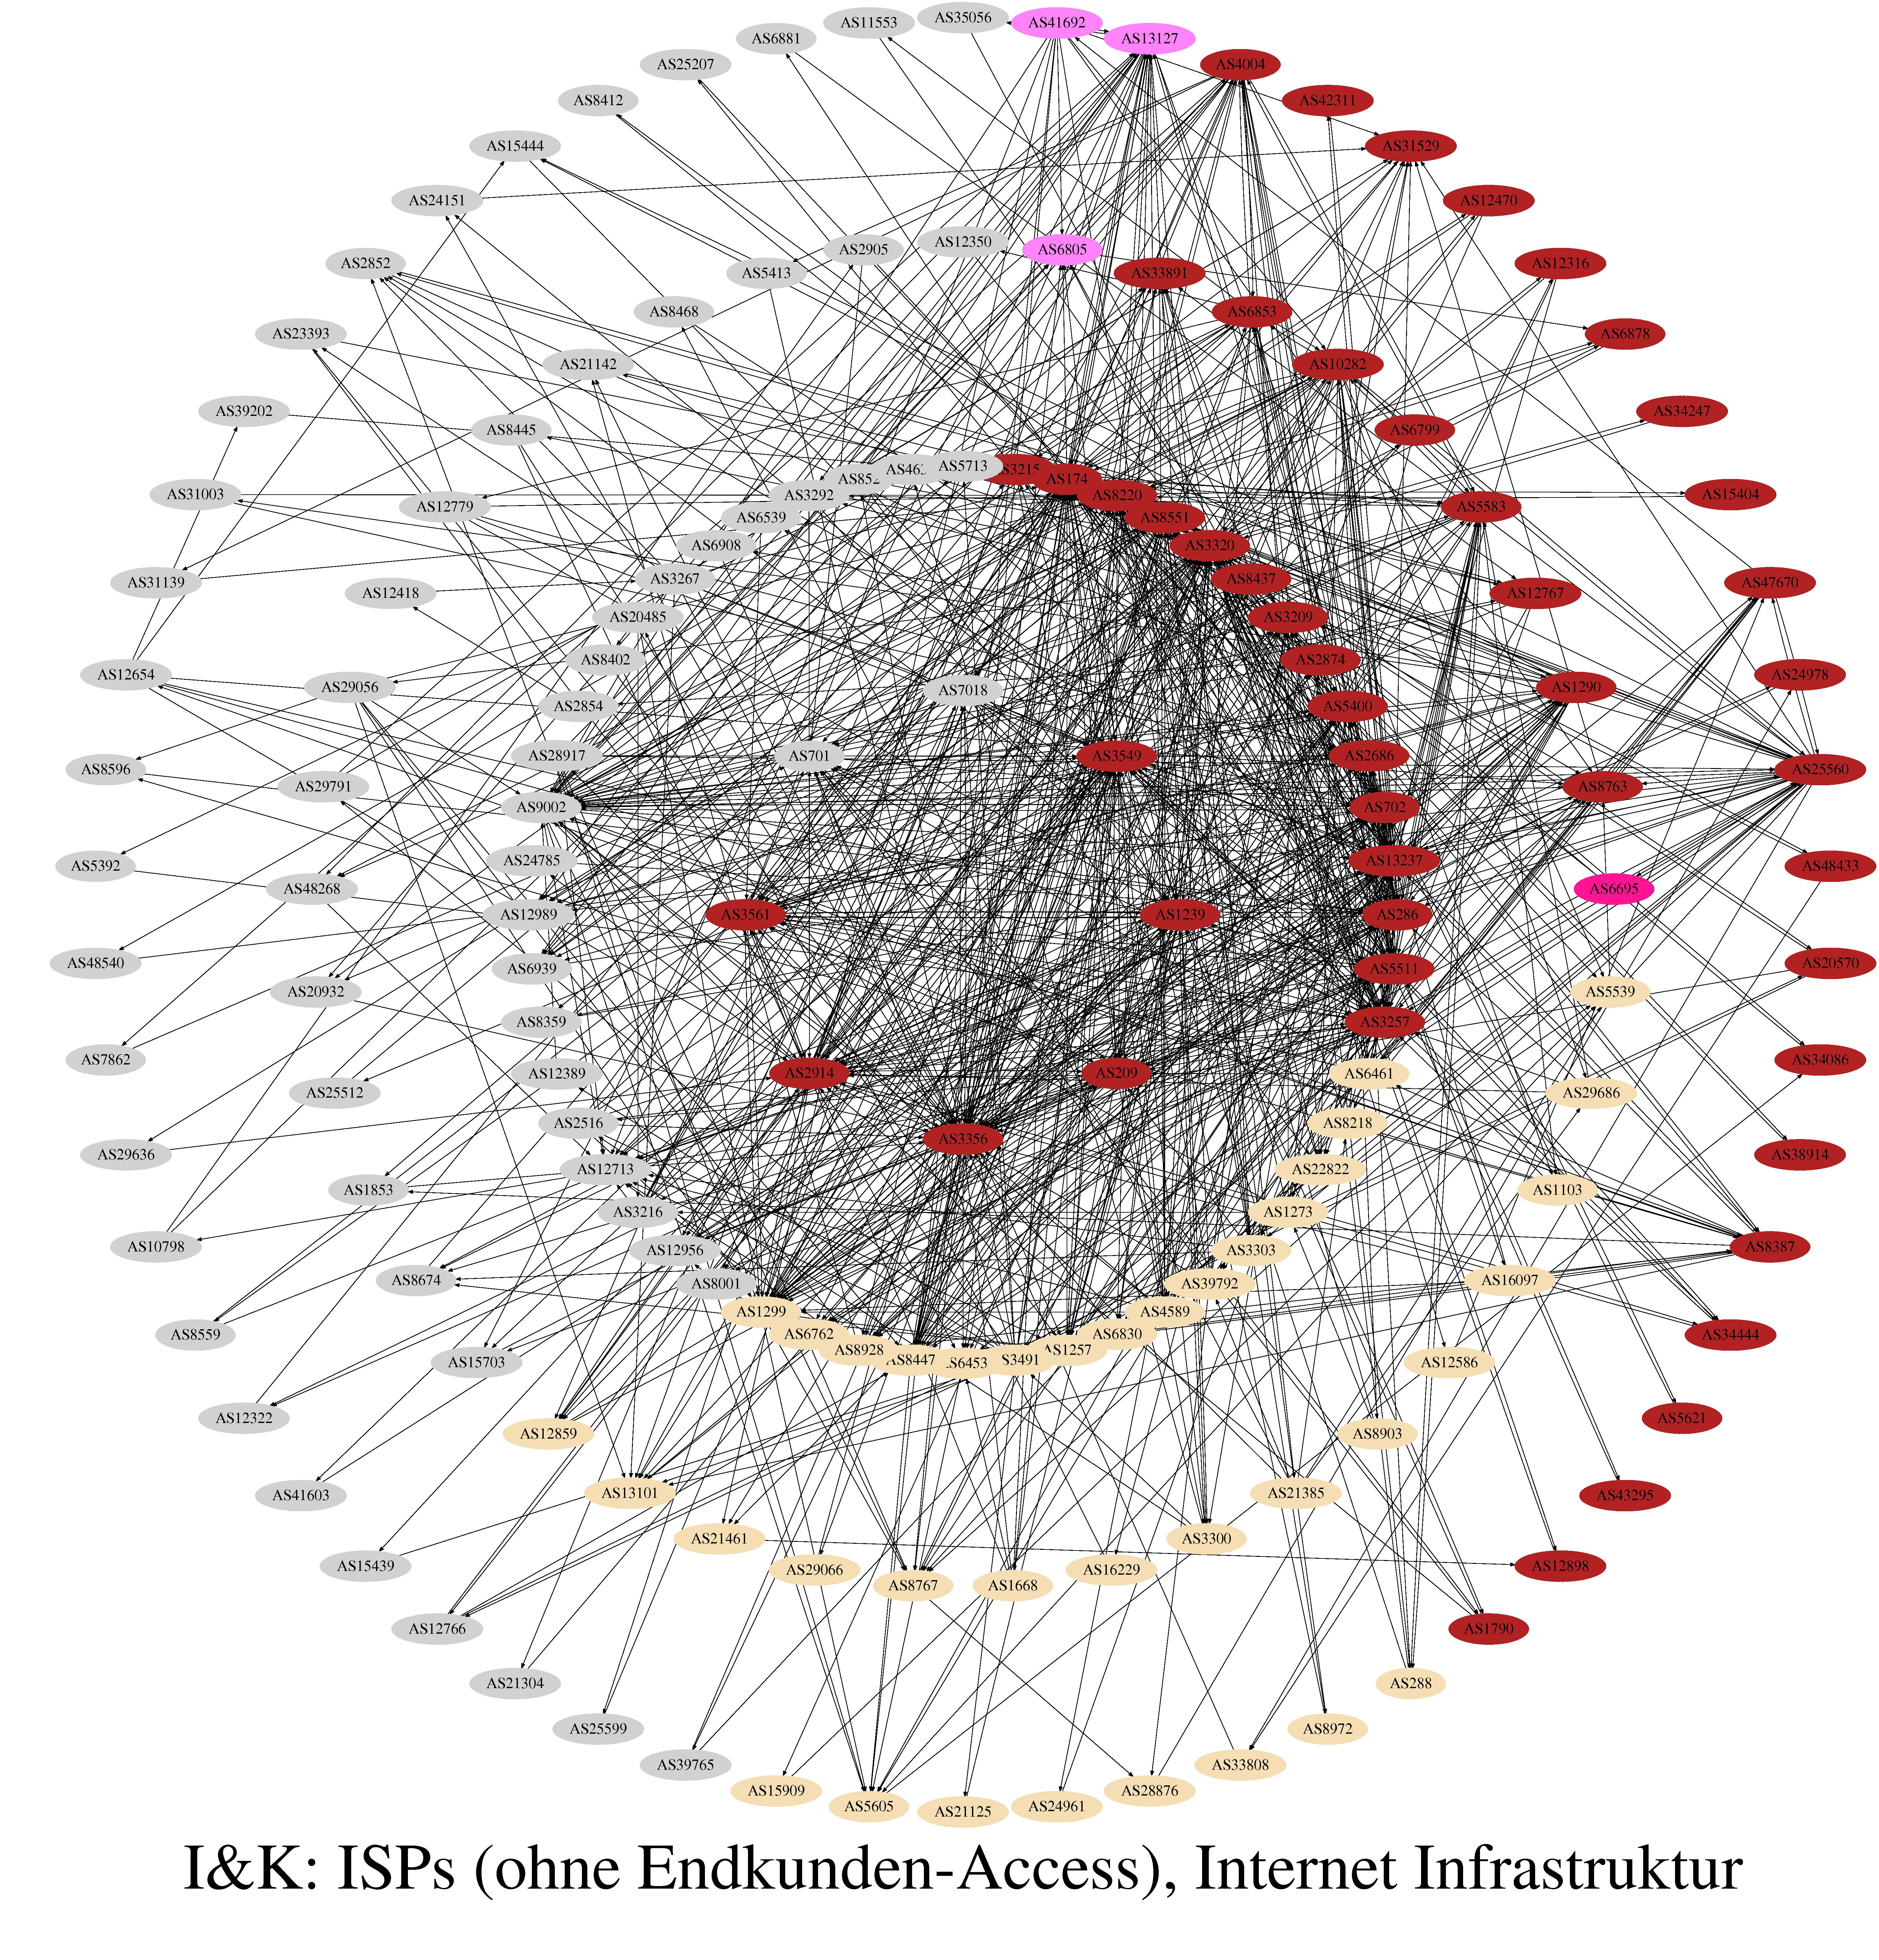
\includegraphics[width=\textwidth]{images/asgraph_cat4-pos}
%  \end{figure}
\end{column}
\end{columns}
\end{frame}

\section{Literatur}
\begin{frame}[plain, allowframebreaks]{Literatur}
\scriptsize
\bibliographystyle{alpha}
\bibliography{folien}
\end{frame}

\section{Bildquellen}
\begin{frame}[plain]{Bildquellen}
  \scriptsize
%   \tiny
  \begin{table}
    \begin{tabular}{ c p{0.8\textwidth} }
      Seite & Quelle \\ \hline
      \pageref{asgraphs}, \pageref{asngraphs2} & \url{http://inet.cpt.haw-hamburg.de/projects/routing-atlas/}\\ \hline
%       & \multirow{3}{0.8\textwidth}{\url{http://www.cs.ucr.edu/~michalis/},\\ \url{http://www.cse.yorku.ca/cspeople/faculty/pfal/index.html},\\ \url{http://www.cs.cmu.edu/~christos/}} \\
%       \pageref{faloutsos}& \\
%       & \\ \hline
      & \multirow{3}{0.8\textwidth}{\url{http://www.cs.arizona.edu/~bzhang/},\\ \url{http://www.cs.colostate.edu/~massey/},\\ \url{http://www.cs.ucla.edu/~lixia/}} \\
      \pageref{zhang_et_al} & \\
      & \\ \hline
%       & \multirow{3}{0.8\textwidth}{\url{http://www.cs.unm.edu/~karlinjf/},\\ \url{http://www.cs.unm.edu/~forrest/},\\ \url{http://www.cs.princeton.edu/~jrex/}} \\
%       \pageref{karlin} & \\
%       & \\ \hline
      & \multirow{4}{0.8\textwidth}{\url{http://www-rp.lip6.fr/~augustin/},\\ \url{http://www.njit.edu/news/2011/2011-054.php},\\ \url{http://www.research.att.com/people/Willinger_Walter/index.html?fbid=Y-QjC_arIwn}} \\
      \pageref{augustin} (rechts) & \\
      & \\ & \\ \hline
      \pageref{augustin_ixp} (l. unten) & \url{http://www-rp.lip6.fr/~augustin/ixp/imc2009.pdf} \\ \hline
      \pageref{gao} & \url{http://www-unix.ecs.umass.edu/~lgao/} \\ \hline
      \pageref{winter} & \url{http://www.hs-augsburg.de/fakultaet/informatik/person/professor/winter_rolf/index.html} \\ \hline
    \end{tabular}
  \end{table}
\end{frame}

\end{document}
